\documentclass[a4paper,12pt,oneside]{article}

% \usepackage{graphicx}
% \usepackage{verbatim}
% \usepackage{amsmath}
% \usepackage[english]{babel}
% \usepackage[colorlinks,bookmarks=false,linkcolor=blue,urlcolor=blue]{hyperref}
% \usepackage{booktabs}

\usepackage{graphicx}
\usepackage{verbatim}
\usepackage{amsmath}
\usepackage[utf8]{inputenc}
\usepackage[colorlinks,bookmarks=false,linkcolor=blue,urlcolor=blue]{hyperref}
\usepackage{booktabs}
\usepackage{subfig}
\usepackage{amssymb}


\paperheight=297mm
\paperwidth=210mm

\setlength{\textheight}{235mm}
\setlength{\topmargin}{-1.2cm}
%\setlength{\footskip}{5mm}
\setlength{\textwidth}{15cm}
\setlength{\oddsidemargin}{0.56cm}
\setlength{\evensidemargin}{0.56cm}

\pagestyle{plain}


\def \be {\begin{equation}}
\def \ee {\end{equation}}
\def \dd  {{\rm d}}

\newcommand{\mail}[1]{{\href{mailto:#1}{#1}}}
\newcommand{\ftplink}[1]{{\href{ftp://#1}{#1}}}


\begin{document}

\title{Physique des couches minces}
\author{Laurent Rohrbasser \& Tim Tuuva}

\maketitle
\tableofcontents
\baselineskip=16pt
\parindent=15pt
\parskip=5pt


\newpage

% \begin{abstract}
% %Résumé de l'expérience, on fait des tps sur le chaos, rappeler vite fait 
% %dire le but de ces manips, qu'est ce qu'on veut?
% \end{abstract}

\section{Introduction}
Il est possible de faire des dépôts de très faibles épaisseur sur des surfaces quelconques relativement lisses. En plus de ne prendre qu'un espace relativement petit, les couches minces ont des propriétés utiles dans le domaine de l'électronique, et la protection aux interfaces d'un autre matériau. Il sera étudié ici les différents résultats de dépot de ZnO par pulvérisation cathodique magnétron sur une plaque de verre pour une variation de la température de dépôt, ainsi que l'effet d'un recuit à différentes températures pour chaque échantillons des couches déposées aux température précédentes.

\section{Un peu de theorie, dipositif expérimental}

Une couche mince, comme son nom l'indique, est une fine couche d'un matériau sur une surface appelée substratqui a généralement une épaisseur variant de $1\AA$ à $10$ micromètres.

Dans les expériences qui suivent, il a été effectué un certain nombre de dépôts de ZnO sur une plaque de verre par pulvérisation cathodique magnétron. Le principe se décrit comme suit (cf fig \ref{fig:illustration_depot}): une cible de ZnO est installée dans une enceinte à vide, le subtrat, ici une plaque de verre, est installée en face, la cible étant exposée à la face sur laquel il est souhaité faire le dépot. Ensuite un gaz réagissant peu (un gaz noble par exemple, ici de l'argon) est introduit dans l'enceinte et une grande différence de potentiel est imposée entre la cible et le substrat. Ceci a pour effet d'arracher un électron de l'argon et donc de le séparer en $Ag^+ + e^-$ et donc d'accélérer les particules $Ag^+$ contre la cible, en transférant de l'energie à la cible, des particules $Zn^+$ et $O^-$ quittent la cible pour se diriger vers la plaque de verre et se recristalliser. Un champ magnétique redirige les particules arrachées de la cible vers la zone où se trouve la plaque de verre. Chaque particule qui arrive sur la surface du verre pourra se déposer en un point et commencer un cluster de particules, se déposer à côté d'une particule ou d'un groupe de particules et ainsi participer à l'agrandissement d'un cluster (cristallisation), diffuser sur la plaque ou réévaporer, ainsi que toutes les combinisons possibles (cf fig \ref{fig:illustration_depot2}).

\begin{figure}[h!]
	\begin{center}
	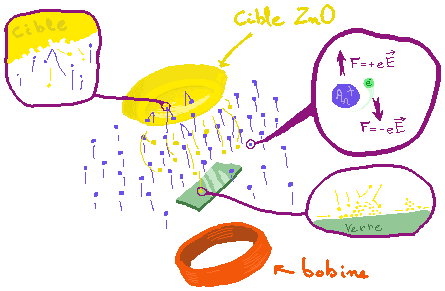
\includegraphics[width=1.\linewidth,angle=0]{./figures/illustration_depot.png}
	\caption{pulvérisation cathodique magnétron} \label{fig:illustration_depot}
	\end{center}
\end{figure}

\begin{figure}[h!]
	\begin{center}
	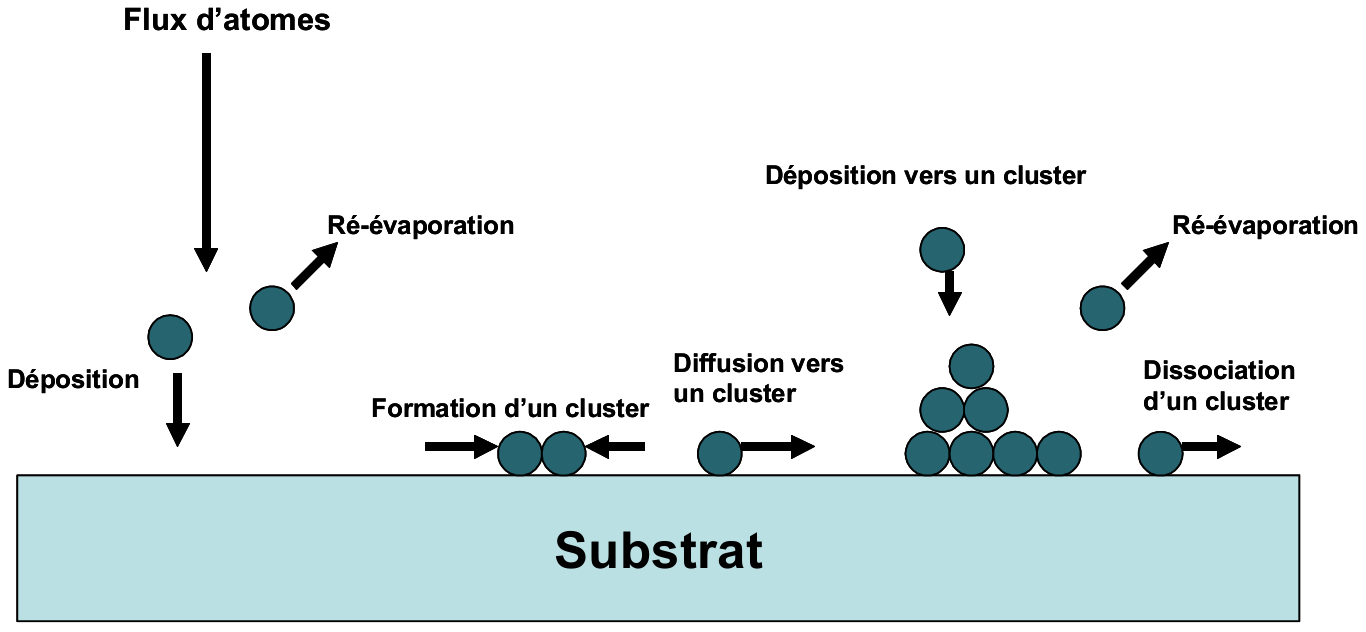
\includegraphics[width=1.\linewidth,angle=0]{./figures/illustration_depot2.png}
	\caption{différentes interractions pour une particule de la cible envoyée sur le substrat, à la surface du substrat} \label{fig:illustration_depot2}
	\end{center}
\end{figure}

Il est assez intuitif qu'il ne va pas se former un seul cristal sans défauts : les clusters peuvent commencer n'importe où avec des orientations différentes, et même au sein des clusters, on aura des défauts de substitution (un atome du cristal est remplacé par un autre atome), interstitielles (un atome se trouve inséré dans une position où on n'atend aucun atome) et lacunes (absence d'atome dans une position où on en attend un). Ces défauts ont des effets différents :

++++++ absence de particule

++++++ remplacement Z

++++++ remplacement O


Dans les dépôts qui sont rélisé ici, on peut aussi considérer le ratio Zn - O : leurs affinités électronique étant différentes, ce ration aura un effet quand à la résistiité de l'échantillon. L'oxygène 
+++ effet de la presence de O dans l'enceinte

+++ ration Zn - O 

++++++ affinite electronique



- expliquer la reformation des microcristaus en un gros cristal a haute temperature
--- pourquoi les gros cristaux grandissent et les petits raptississent ?

- pourquoi depot a chaud change
--- energie de la plaque de verre transmise dans les particules de Zn, ainsi les Zn regagnent de l'energie et peuvent se mettre dans des endroits ou leur potentiel est plus faible.

differents depots : Temperature
	- change l'energie fournue a la particule envoyee sur le substrat (favorise la formation de gros cristaux)
recuit
	- change la taille des cristaux (recristalisation)


semiconducteur
	- gap $\delta$V
	- P ou N
les choses qu'on peut faire avec
	- diode shotzky
	- diode normale
	- diode photovoltaique (transparence de la couche)

\subsection{resistivite (methode Van der Pauw)}
	La méthode devan der Pauw fonctionne sur des échantillons plats, homogène et de faible épaisseur. On prends 4 points de contacts comme dans la figure \ref{fig:illustration_van_der_pauw}, et on applique sur toutes les combinaisons possibles un courant et on mesure la tension entre les autres contacts restant (à un signe près) ce qui permet de calculer la résistivité avec la relation
	\be
		\rho = \frac{\pi}{ln 2} d R_{moyen}  F(R_1/R_2)
	\ee
	où d est l'épaisseur de l'échantillon, $R_{moyen}$ la moyenne des $R_1=V_{34}/I_{12}$ , $R_2=V_{41}/I_{23}$ , $R_3=V_{12}/I_{34}$ et $R_4=V_{23}/I_{41}$ et F est un facteur de correction pour un cas asymétrique, qui vaut 1 si le montage est réalisé comme dans la figure.
		\begin{figure}[h!]
			\begin{center}
			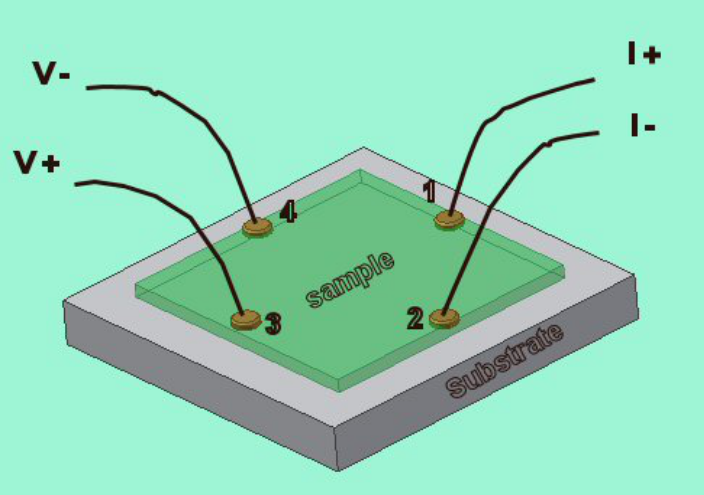
\includegraphics[width=.5\linewidth,angle=0]{./figures/illustration_van_der_pauw.png}
			\caption{Les contacts sont sur les sommets d'un carré pour avoir des distances identiques entre 1-3 et 2-4 ainsi que 1-2 et 2-3 et 3-4 et 4-1} \label{fig:illustration_van_der_pauw}
			\end{center}
		\end{figure}

\subsection{profilometre}
	Le profilomètre sert à simplement mesurer l'épaisseur des échantillons en faisant un balayage entre une surface qui a un dépôt et une surface qui a été converte pendant le dépôt (où il n'y a pas de couche mince donc) et qui va mesurer les variations de l'épaisseur.

\subsection{Effet Hall}
	L'effet Hall est la création d'une différence de potentiel lorsqu'on fait passer un courant dans un échantillon plongé dans un champ magnétique. La force de Lorentz appliquée aux électrons qui circulent dans l'échantillon implique une déviation des charges sur le côté et donc une différence de potentiel dans la direction orthogonale au courant (il faut que le champ ne soit pas aligné avec le courant).

	De la relation
	\be
		U_H = \frac{IB}{qNd}
	\ee
	où I est le courant imposé, B la valeur du champ lorsque celui ci est orthogonal à B, q la charge déplacée, d l'épaisseur de l'échantillon et N la densité de porteur de charges.

	Il est ainsi possible de calculer $N$ ainsi que la mobilité $\mu$ des porteurs de charge grâce à la relation
	\be
		\sigma = q N \mu
	\ee

\subsection{spectre de reflexion}
% coeff absorption
% gap optique

L'expérience consiste en envoyer de la lumière d'un spectre assez large, et voir ce qui est réfléchi.

\be
	\omega_{min}=\sqrt{ \frac{q^2 N_{opt}} {\epsilon_0(\epsilon_\infty-1)m^*} }
\ee

ou $m^*$ est la masse effective de l'électron ($0.35 m_e$ pour le ZnO),

% \subsection{spectre de transmission}



\subsection{Diffraction rayonX}













\section{résultats des expériences}

L'idée est de faire des dépôts à différentes températures pour observer vers quel état final tend la couche mince obtenue : il sera donc mesuré et comparé résistivité, épaisseur, taille des cristaux formés et densité de porteurs de charges libres par les méthodes décrites précédemment. Il sera aussi comparé les effets de recuits à différentes température.

Note : Dans l'ensemble des expérience, il a été ajouté dans l'enceinte du pulvérisateur cathodique magnétron un peu d'oxygène afin de rétablir la stoechiométrie pour le cristal ZnO : en effet, l'oxygène étant plus volatile que le zinc, on se retrouve avec un déficit en O. Malheureusement, le gaz introduit n'était pas purement de l'oxygène, mais une composition $21 \% O_2 $ et $78 \% N_2 $ et $1 \% $ de diverses impuretés.

+++ la temperature dans l'enceinte augmente avec le plasma

\subsection{resistivite (methode Van der Pauw)}

\subsection{profilometre}

\subsection{Effet Hall}

L'expérience a causé un problème quand à la mesurabilité de l'effet : il n'a pas été possible de dinstinguer la différence de potentiel entre le moment où le champ magnétique était imposé et le moment où il n'y en avait pas, les variations étant plus faible que le bruit des appareils de mesure, il était impossible d'obtenir une variation de U. Le seul indice qu'il a pu être obtenu est que pour un champ de 1 Tesla, un courant de 32 mA (maximum qui a pu être imposé), les variations par rapport à un champ nul étaient en dessous de 0.001 mV. En plus de cela, les valeurs ne convergeant pas (l'échantillon chauffe) et il est pourtant nécessaire d'attendre après activation du champ magnétique car le bruit explose à ce moment.


\subsection{spectre de reflexion}


% \subsection{spectre de transmission}
% n'a pas pu être réalisé.

\subsection{Diffraction rayonX}








% 1:
% 2:
% 3: Zn + O2






% [x] A0 dépot 20° (No O2)
% [x] Ax dépot 20° (No O2) + recuit 400°

% [x] A1 dépot 20°
% [x] A2 dépot 20° + recuit 400°
% [x] A3 dépot 20° + recuit 600°

% [x] B1 dépot 200°
% [x] B2 dépot 200° + recuit 600°

% [x] C1 dépot 400°
% [x] C2 dépot 400° + recuit 600°



% résistivité
% [x]A0
% [ ]Ax
% [x]A1
% [ ]A2
% [ ]A3
% [ ]B1
% [ ]B2
% [x]C1
% [ ]C2

% épaisseur (profilomètre)
% [x]A0
% [!]Ax
% [x]A1
% [!]A2
% [!]A3
% [x]B1
% [!]B2
% [x]C1
% [!]C2

% concentration charge par effet Hall
% [?]A0
% [?]Ax
% [?]A1
% [?]A2
% [?]A3
% [?]B1
% [?]B2
% [?]C1
% [?]C2

% Spectre
% [x]A0
% [x]Ax
% [x]A1
% [ ]A2
% [x]A3
% [x]B1
% [x]B2
% [x]C1
% [x]C2

% Diffraction 
% [ ]A0
% [ ]Ax
% [ ]A1
% [ ]A2
% [ ]A3
% [ ]B1
% [ ]B2
% [ ]C1
% [ ]C2




%Exposition des graphes avec les légendes et un peu de texte explicatifs sur comment on les a obtenus.

% \begin{figure}[h!]
%   \begin{center}
%   %\includegraphics[width=0.8\linewidth,angle=0]{}
%   \caption{} \label{fig:}
%   \end{center}
% \end{figure}

\section{Discussion}%le plus important

\subsection{Interprétation}
%Qu'est ce que les résultats nous permettent de conclure?
%Est ce que cela nous aide pour nôtre but?

\section{Conclusion}

%Résumer du rapport
%Ouverture





%Reference
\begin{thebibliography}{99}
\bibitem{la notice}
\end{thebibliography}

\end{document}
